\documentclass[tikz, border=2mm]{standalone}
\usepackage{amsmath}

\begin{document}
	
	% ដាក់កូដ TikZ របស់អ្នកនៅទីនេះ (ឧទាហរណ៍ សំណួរទី៨)
	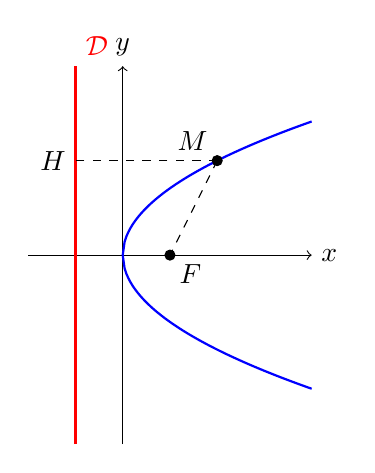
\begin{tikzpicture}[scale=0.6]
		% Axes
		\draw[->] (-2,0) -- (4,0) node[right] {$x$};
		\draw[->] (0,-4) -- (0,4) node[above] {$y$};
		
		% Parabola
		\draw[thick, blue, domain=0:4, samples=100] plot (\x, {sqrt(2*\x)});
		\draw[thick, blue, domain=0:4, samples=100] plot (\x, {-sqrt(2*\x)});
		
		% Directrix
		\draw[red, thick] (-1,-4) -- (-1,4) node[above right] {$\mathcal{D}$};
		
		% Points
		\filldraw[black] (1,0) circle (3pt) node[below right] {$F$};
		\filldraw[black] (2,2) circle (3pt) node[above left] {$M$};
		
		% Dashed lines
		\draw[dashed] (2,2) -- (-1,2) node[left] {$H$};
		\draw[dashed] (2,2) -- (1,0);
	\end{tikzpicture}
	
\end{document}